\chapter{Fill Reducing Reordering}
\label{app:app-fill-reducing-reodering}



\figpointer{\ref{fig:mumps-ordering-2}}
\begin{figure}[htpb]
\centering
	\begin{tabular}{cc}
		\subfloat[cube-5]{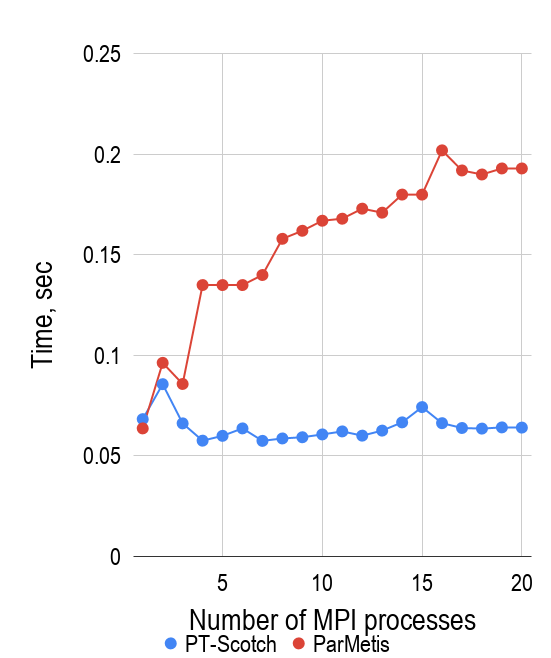
\includegraphics[width=0.48\textwidth]{figures/chapter-2/ordering/cube-5.png}} &
		\subfloat[cube-645]{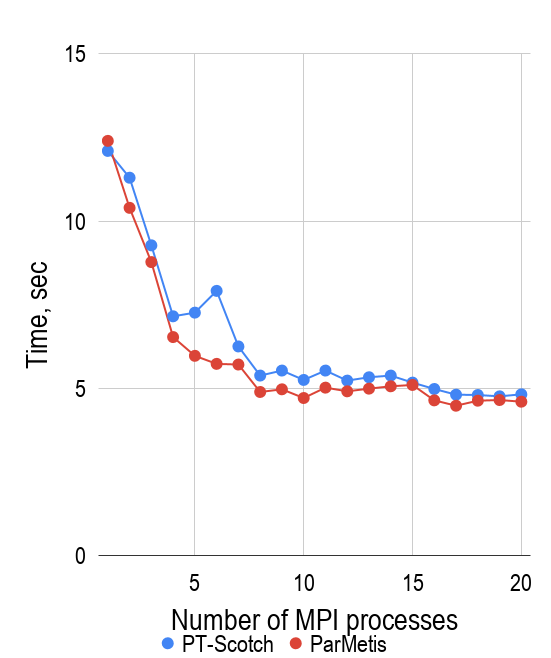
\includegraphics[width=0.48\textwidth]{figures/chapter-2/ordering/cube-645.png}} \\
		\subfloat[cant]{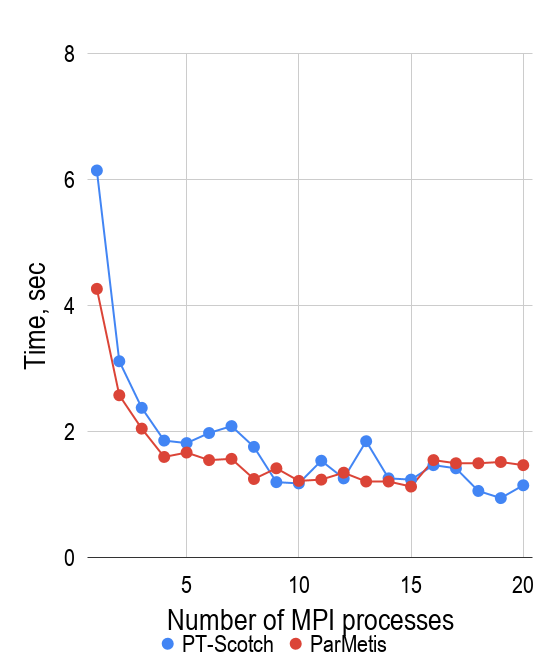
\includegraphics[width=0.48\textwidth]{figures/chapter-2/ordering/cant.png}} &
		\subfloat[memchip]{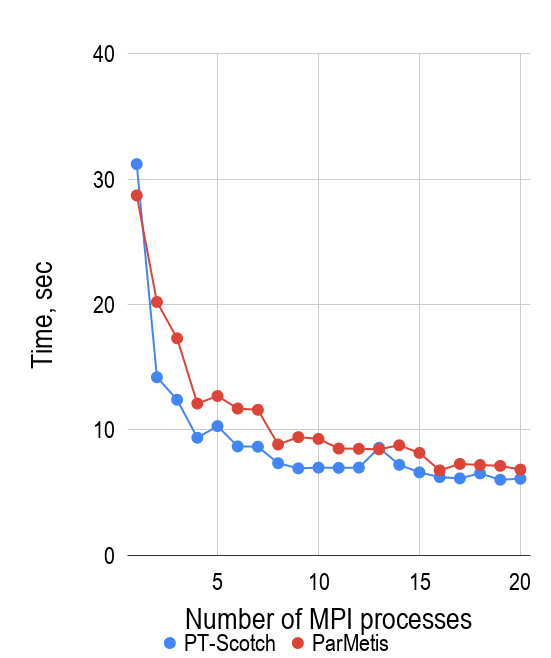
\includegraphics[width=0.48\textwidth]{figures/chapter-2/ordering/memchip.png}} \\
	\end{tabular}
	\caption{An influence of different fill-reducing algorithms on parallel factorizations of \textit{cube-5}, \textit{cube-645}, \textit{cant} and \textit{memchip}}
	\label{fig:mumps-ordering-2}
\end{figure}




\figpointer{\ref{fig:mumps-ordering-3}}
\begin{figure}[htpb]
\centering
	\begin{tabular}{cc}
		\subfloat[torso3]{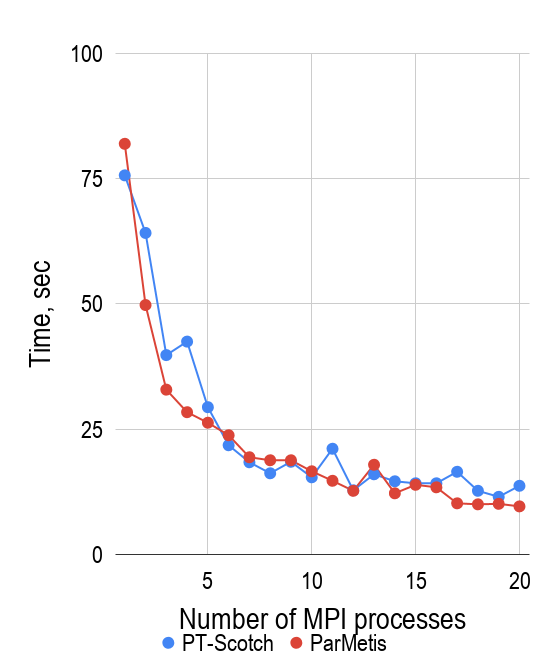
\includegraphics[width=0.48\textwidth]{figures/chapter-2/ordering/torso3.png}} &
		\subfloat[consph]{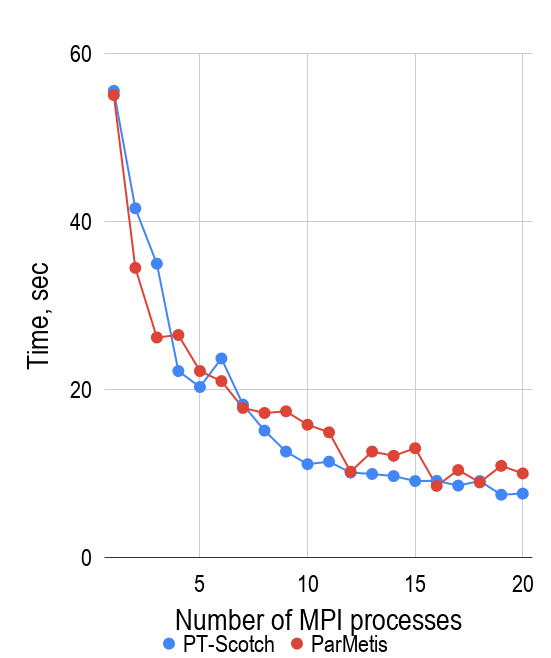
\includegraphics[width=0.48\textwidth]{figures/chapter-2/ordering/consph.png}} \\
		\subfloat[CurlCurl\_3]{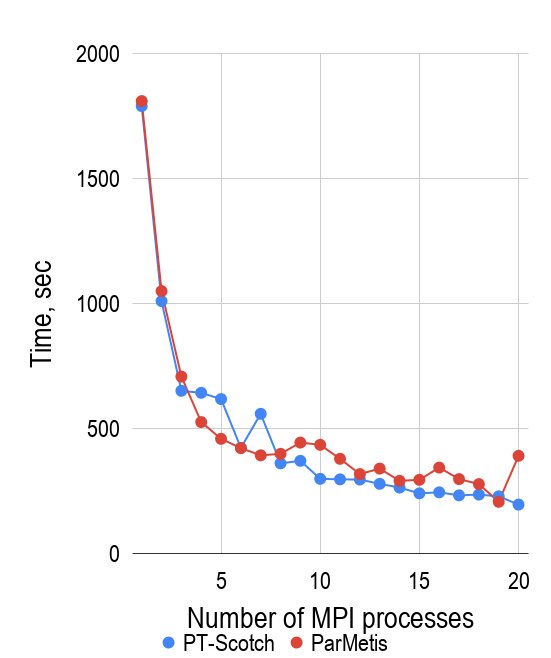
\includegraphics[width=0.48\textwidth]{figures/chapter-2/ordering/CurlCurl_3.png}} &
		\subfloat[x104]{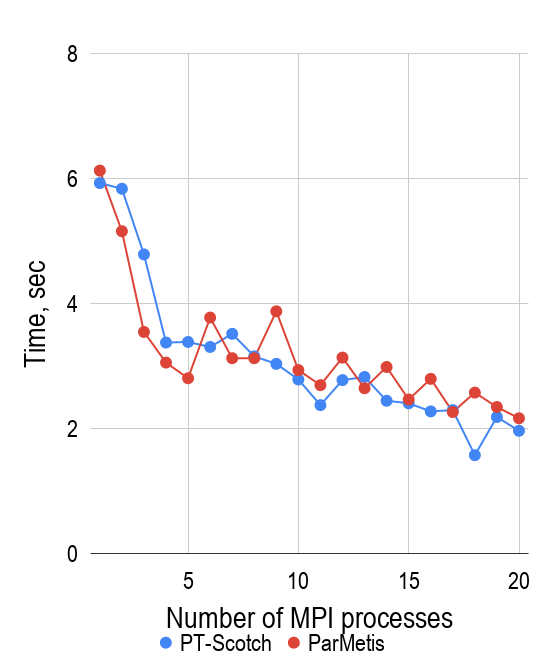
\includegraphics[width=0.48\textwidth]{figures/chapter-2/ordering/x104.png}} \\
	\end{tabular}
	\caption{An influence of different fill-reducing algorithms on parallel factorizations of \textit{torso3}, \textit{consph}, \textit{CurlCurl\_3} and \textit{x104}}
	\label{fig:mumps-ordering-3}
\end{figure}